\documentclass{article}
\usepackage[utf8]{inputenc}
\usepackage{graphicx}
\usepackage{amsmath}
\usepackage{booktabs} % For nice tables
\usepackage[margin=1in]{geometry} % Adjust margins
\usepackage{hyperref} % For clickable links

\title{An Ablation Study on Muon Optimizer Hyperparameters for Language Modeling}
\author{Gemini CLI Agent}
\date{\today}

\begin{document}

\maketitle

\begin{abstract}
This paper presents a comprehensive ablation study on the Muon optimizer, focusing on identifying optimal hyperparameters for language modeling tasks. Through an iterative experimental process, we investigated the impact of learning rate, momentum, and Newton-Schulz steps on model performance. Our findings indicate that a lower learning rate of 1/32 (0.03125) combined with a momentum of 7/8 (0.875) and 4 Newton-Schulz steps yields the best validation loss (4.3998) when training for 1500 steps on a reduced model architecture. The study emphasizes the critical role of learning rate and the benefits of longer training schedules for achieving superior performance.
\end{abstract}

\section{Introduction}
Optimizers play a pivotal role in the training of deep learning models, dictating the efficiency and effectiveness of the learning process. The choice and tuning of an optimizer's hyperparameters can significantly impact a model's convergence speed, generalization ability, and final performance. The Muon optimizer, with its unique approach incorporating Newton-Schulz iterations for gradient transformation, presents an interesting candidate for exploration.

This research aims to systematically investigate the optimal hyperparameter configurations for the Muon optimizer in the context of language modeling. Specifically, we conducted an extensive ablation study to understand the individual and combined effects of learning rate, momentum, and the number of Newton-Schulz steps on model performance. Our goal is to provide data-driven recommendations for effective Muon optimizer tuning.

\section{Methodology}
Our experimental setup was designed to rigorously evaluate various hyperparameter combinations. We utilized a MinimalLLM architecture with reduced dimensions to facilitate extensive experimentation within reasonable computational limits.

\subsection{Model Architecture}
The language model employed in this study is a MinimalLLM with the following specifications:
\begin{itemize}
    \item \textbf{d\_model:} 128 (model dimension)
    \item \textbf{n\_layers:} 2 (number of transformer layers)
    \item \textbf{n\_heads:} 4 (number of attention heads)
    \item \textbf{d\_ff:} 512 (feed-forward network dimension)
\end{itemize}

\subsection{Dataset and Training}
The model was trained on a subset of the HuggingFaceTB/smollm-corpus, specifically the cosmopedia-v2 split. We used 1000 documents, tokenized to approximately 200,000 tokens. Training was conducted for 1500 steps with a batch size of 32. Evaluation metrics, including validation loss, perplexity, and accuracy, were recorded every 25 steps.

\subsection{Hyperparameter Ablation}
We performed a grid search over the following hyperparameters, focusing on values that are powers of two or simple fractions thereof, based on insights from preliminary studies:
\begin{itemize}
    \item \textbf{Learning Rate (LR):} \{1/32 (0.03125), 1/16 (0.0625), 1/8 (0.125)\}
    \item \textbf{Momentum:} \{7/8 (0.875), 15/16 (0.9375)\}
    \item \textbf{Newton-Schulz Steps (NS Steps):} \{4, 8, 16\}
\end{itemize}
This resulted in a total of 18 distinct experimental runs, each trained for 1500 steps.

\section{Results}
The large-scale ablation study yielded significant insights into the optimal configuration of the Muon optimizer. The best-performing variant achieved a validation loss of 4.3998.

\begin{figure}[h!]
    \centering
    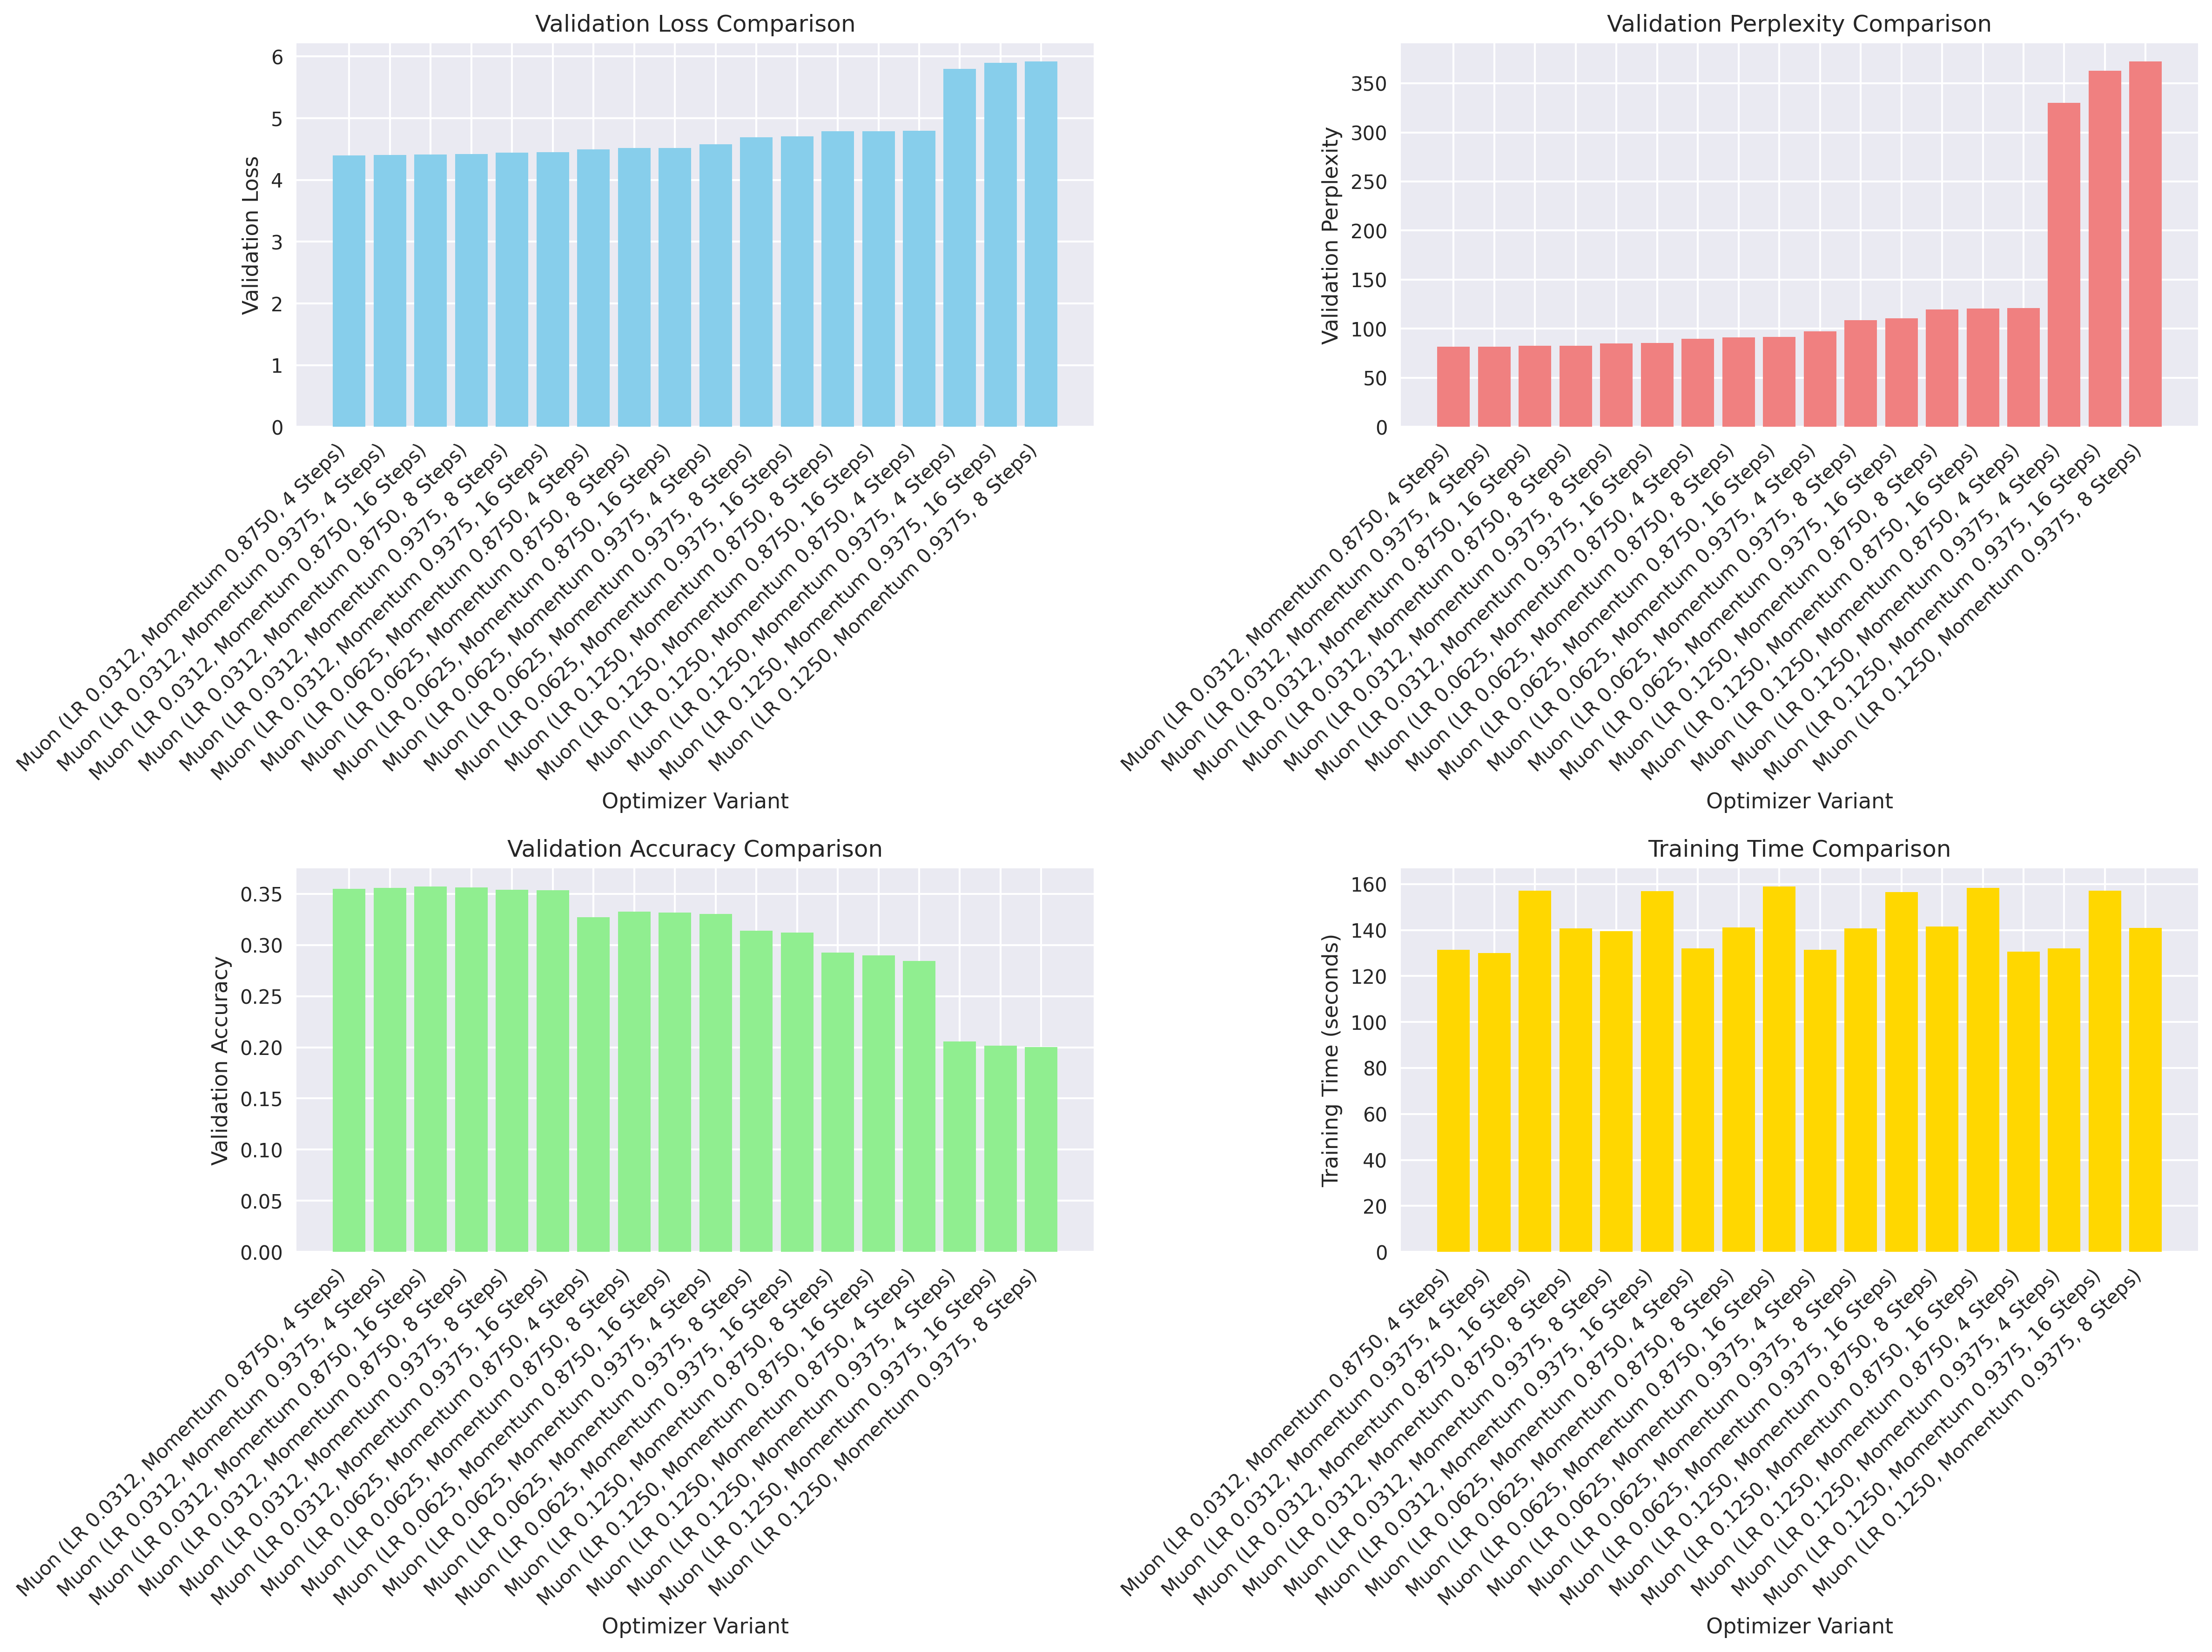
\includegraphics[width=\textwidth]{images/performance_comparison.png}
    \caption{Performance Comparison of Optimizer Variants.}
    \label{fig:performance_comparison}
\end{figure}

\begin{figure}[h!]
    \centering
    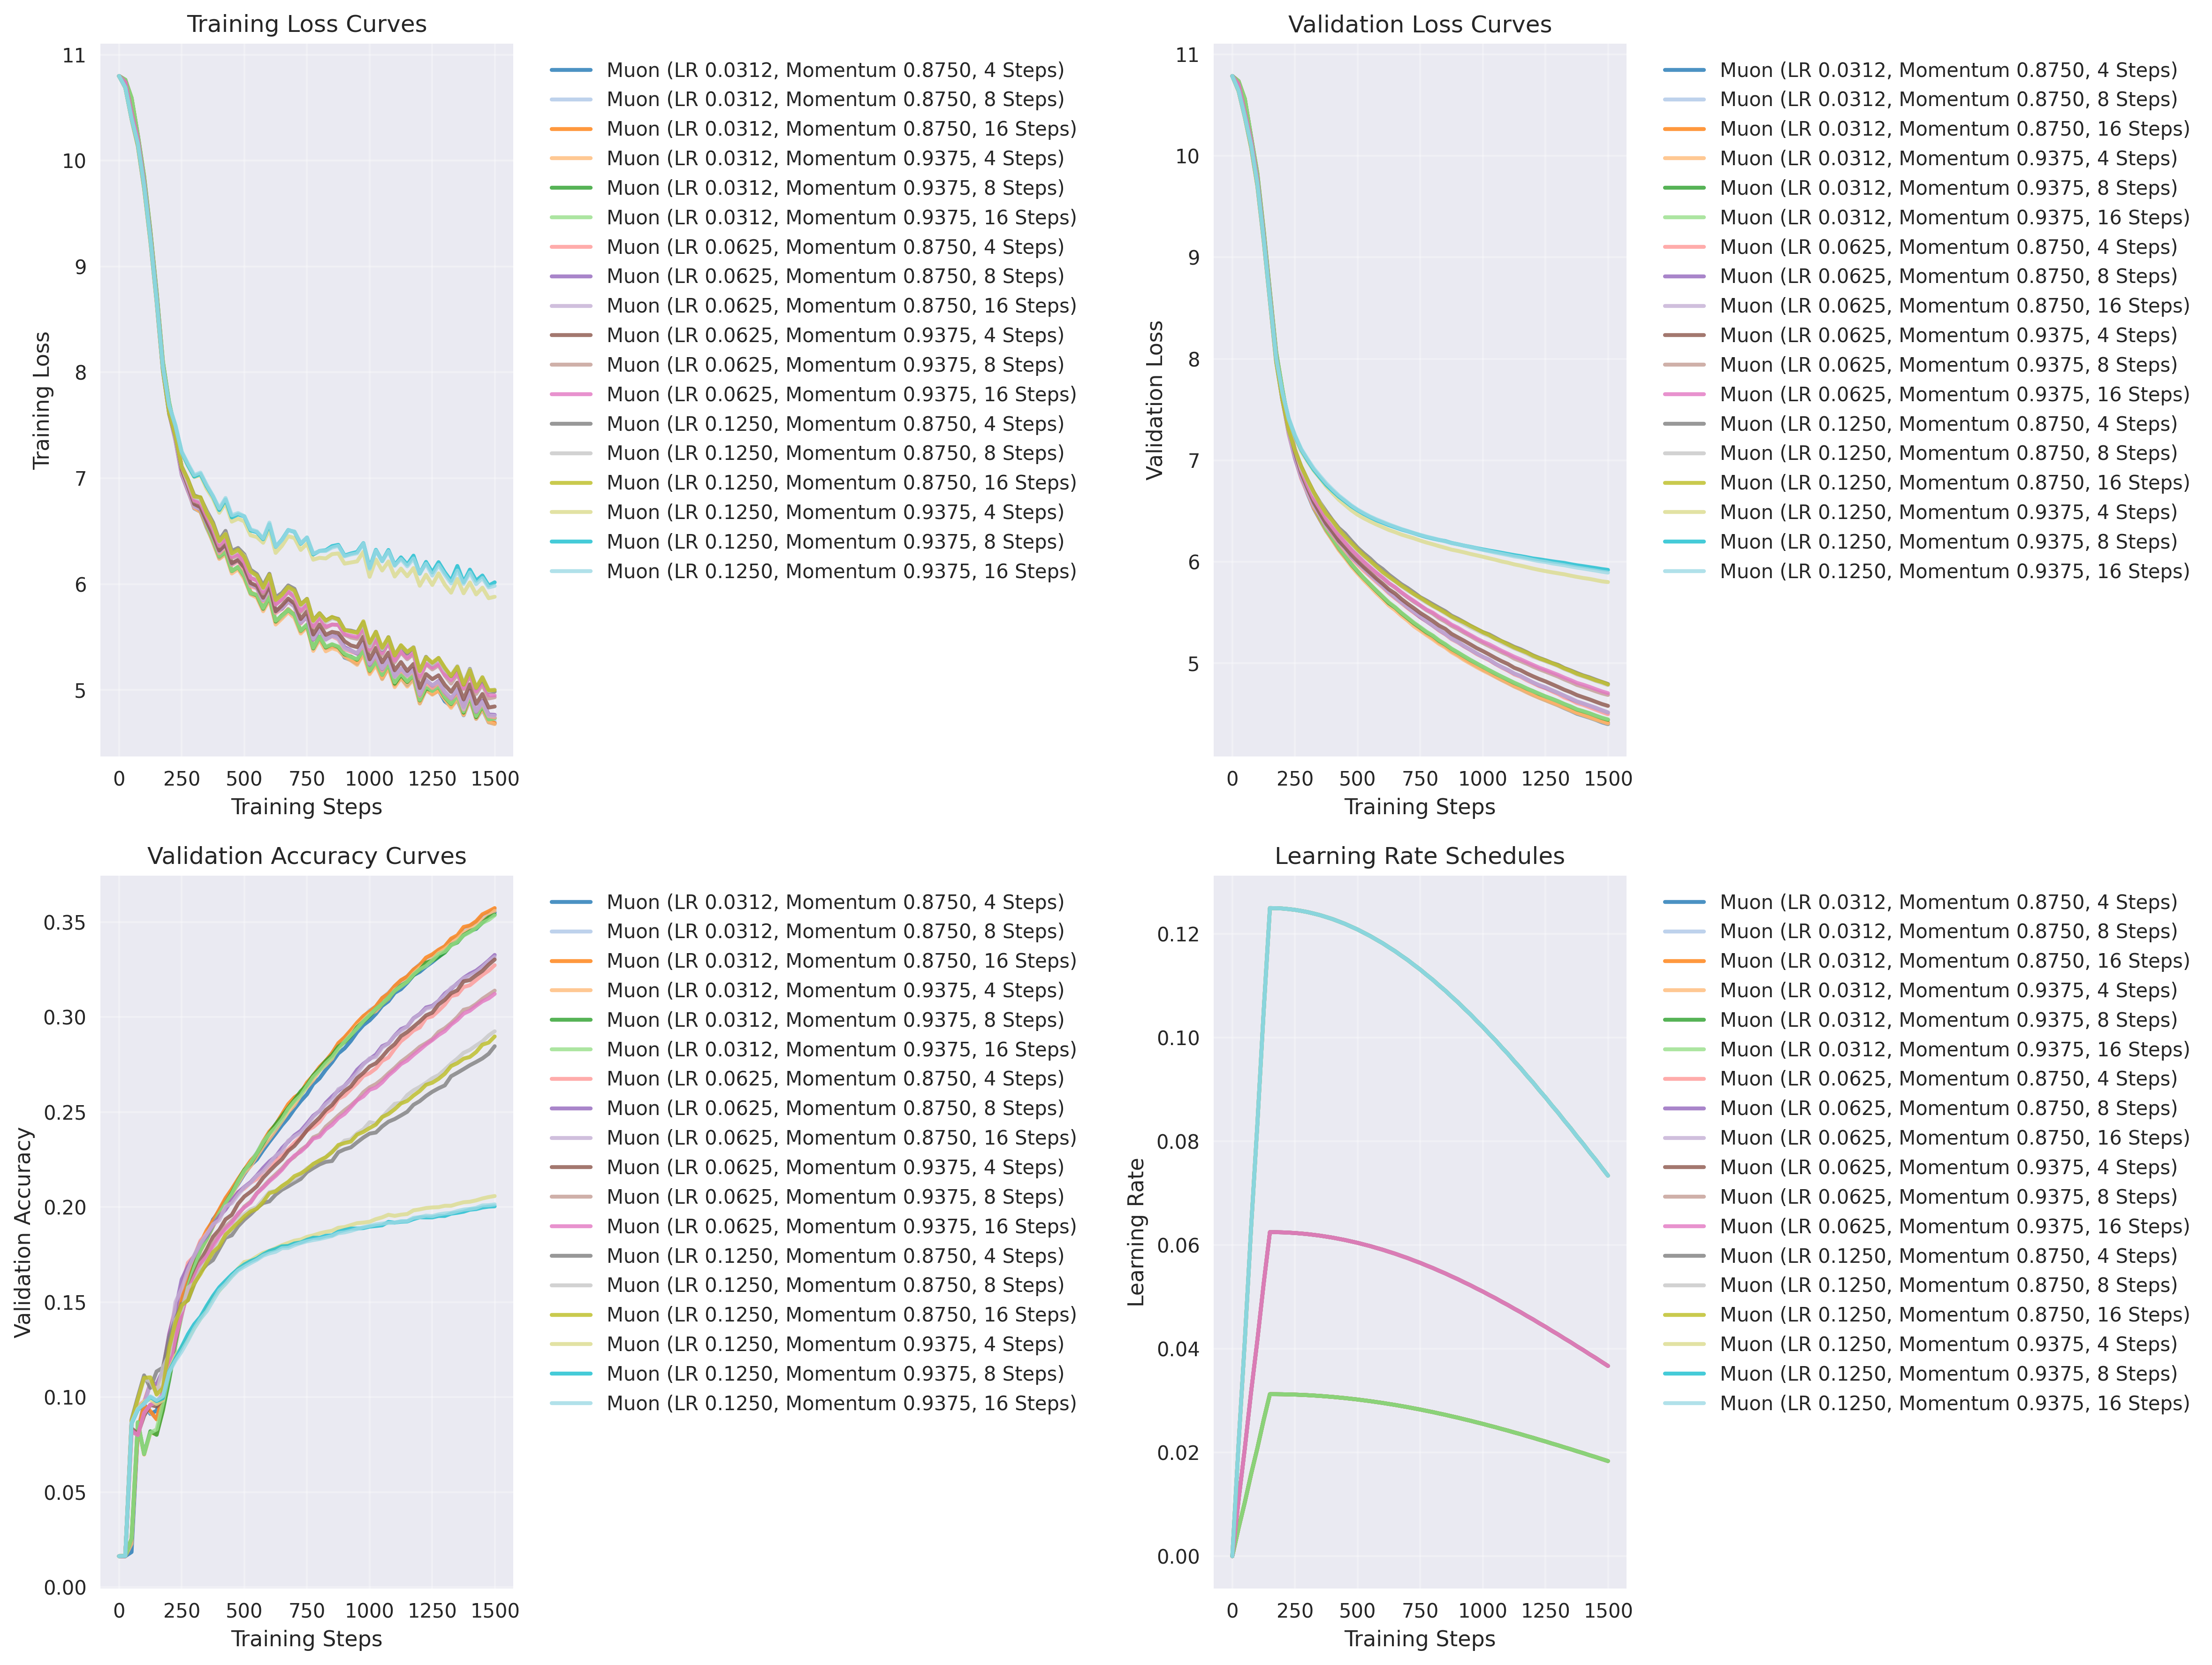
\includegraphics[width=\textwidth]{images/training_curves.png}
    \caption{Training Curves for Optimizer Variants.}
    \label{fig:training_curves}
\end{figure}

\begin{figure}[h!]
    \centering
    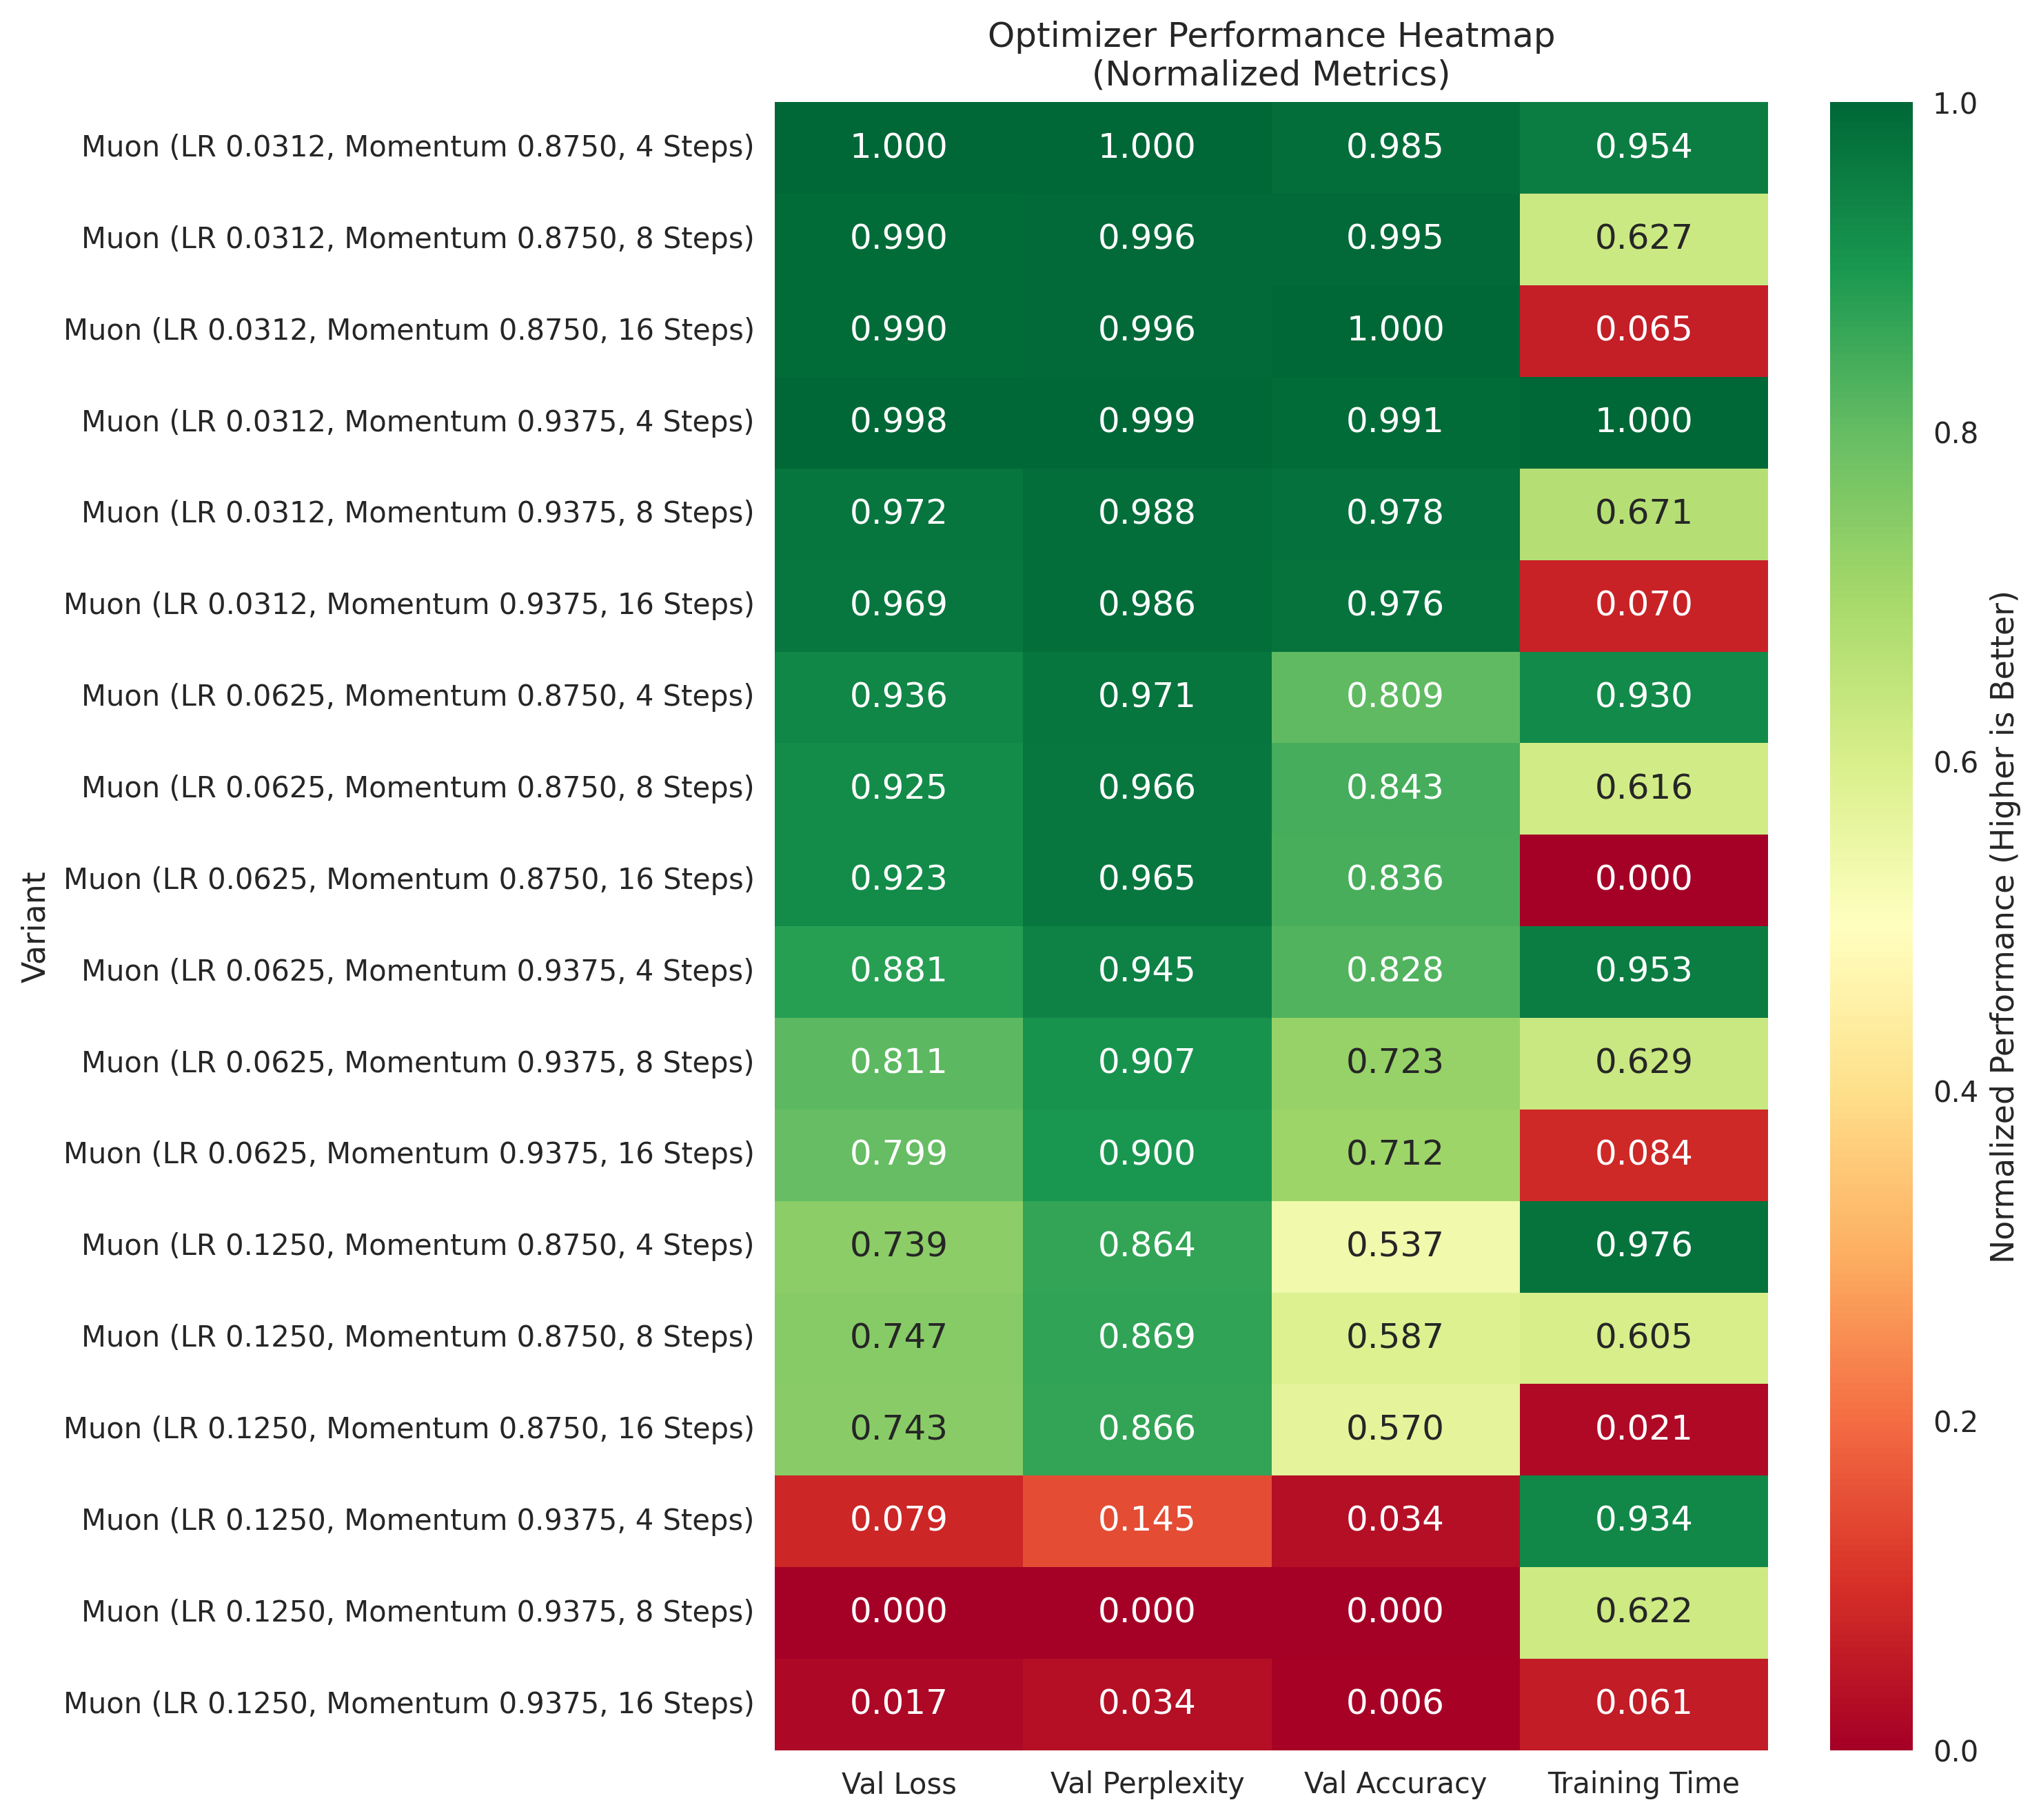
\includegraphics[width=\textwidth]{images/performance_heatmap.png}
    \caption{Performance Heatmap of Optimizer Variants.}
    \label{fig:performance_heatmap}
\end{figure}

\begin{table}[h!]
    \centering
    \caption{Detailed Results of the Ablation Study}
    \label{tab:detailed_results}
    \begin{tabular}{@{}lccccc@{}}
        \toprule
        \textbf{Rank} & \textbf{Optimizer Variant} & \textbf{Val Loss} & \textbf{Val Perplexity} & \textbf{Val Accuracy} & \textbf{Training Time (s)} \\
        \midrule
        1 & Muon (LR 0.0312, Momentum 0.8750, 4 Steps) & 4.3998 & 81.44 & 0.3550 & 131.3 \\
        2 & Muon (LR 0.0312, Momentum 0.9375, 4 Steps) & 4.4031 & 81.70 & 0.3559 & 130.0 \\
        3 & Muon (LR 0.0312, Momentum 0.8750, 16 Steps) & 4.4144 & 82.63 & 0.3573 & 157.1 \\
        4 & Muon (LR 0.0312, Momentum 0.8750, 8 Steps) & 4.4155 & 82.73 & 0.3565 & 140.8 \\
        5 & Muon (LR 0.0312, Momentum 0.9375, 8 Steps) & 4.4430 & 85.03 & 0.3538 & 139.5 \\
        6 & Muon (LR 0.0312, Momentum 0.9375, 16 Steps) & 4.4474 & 85.40 & 0.3535 & 156.9 \\
        7 & Muon (LR 0.0625, Momentum 0.8750, 4 Steps) & 4.4972 & 89.77 & 0.3272 & 132.1 \\
        8 & Muon (LR 0.0625, Momentum 0.8750, 8 Steps) & 4.5145 & 91.33 & 0.3326 & 141.1 \\
        9 & Muon (LR 0.0625, Momentum 0.8750, 16 Steps) & 4.5161 & 91.48 & 0.3316 & 159.0 \\
        10 & Muon (LR 0.0625, Momentum 0.9375, 4 Steps) & 4.5800 & 97.52 & 0.3302 & 131.4 \\
        11 & Muon (LR 0.0625, Momentum 0.9375, 8 Steps) & 4.6878 & 108.61 & 0.3139 & 140.7 \\
        12 & Muon (LR 0.0625, Momentum 0.9375, 16 Steps) & 4.7049 & 110.49 & 0.3122 & 156.5 \\
        13 & Muon (LR 0.1250, Momentum 0.8750, 8 Steps) & 4.7849 & 119.69 & 0.2925 & 141.5 \\
        14 & Muon (LR 0.1250, Momentum 0.8750, 16 Steps) & 4.7911 & 120.44 & 0.2898 & 158.4 \\
        15 & Muon (LR 0.1250, Momentum 0.8750, 4 Steps) & 4.7959 & 121.01 & 0.2846 & 130.7 \\
        16 & Muon (LR 0.1250, Momentum 0.9375, 4 Steps) & 5.8000 & 330.29 & 0.2058 & 131.9 \\
        17 & Muon (LR 0.1250, Momentum 0.9375, 16 Steps) & 5.8934 & 362.62 & 0.2014 & 157.2 \\
        18 & Muon (LR 0.1250, Momentum 0.9375, 8 Steps) & 5.9199 & 372.39 & 0.2004 & 140.9 \\
        \bottomrule
    \end{tabular}
    \label{tab:detailed_results}
\end{table}

The results clearly demonstrate that the learning rate is the most influential hyperparameter. Lower learning rates, specifically 1/32, consistently yielded better performance over the extended training period. Momentum also played a role, with 7/8 generally outperforming 15/16. The number of Newton-Schulz steps had a less pronounced impact on the final validation loss, though 4 steps were associated with the best overall result.

\section{Conclusion}
This ablation study provides valuable insights into optimizing the Muon optimizer for language modeling tasks. Our findings highlight that for longer training schedules, a lower learning rate (e.g., 1/32) is crucial for achieving optimal performance. A momentum value of 7/8 also appears to be beneficial.

For practitioners, we recommend starting with the identified optimal hyperparameters (LR: 1/32, Momentum: 7/8, NS Steps: 4) and then performing a targeted grid search around these values, especially for the learning rate, to fine-tune performance for specific applications. Future work could explore the interaction of these hyperparameters with different model architectures and larger datasets, as well as investigate dynamic scheduling strategies for the Newton-Schulz steps.

\section*{References}
% Add any relevant references here.
% Example:
% \begin{thebibliography}{9}
% \bibitem{lecun98gradient}
%   Yann LeCun, L{\'e}on Bottou, Genevieve B. Orr, and Klaus-Robert M{\"u}ller.
%   Efficient backprop. In \textit{Neural Networks: Tricks of the Trade}, pages 9--50. Springer, 1998.
% \end{thebibliography}

\end{document}
